\chapter{Señal de Televisión}

\section{Banda de TV y Radio FM}
Las frecuencias portadoras para los canales de televisión VHF 2-4 cubre el rango de frecuencia de 54 a 72 MHz. Hay una banda de 72-76 MHz que está reservada para servicios gubernamentales y no gubernamentales, incluyendo una radiobaliza aeronáutica estándar a 75 MHz. Los canales de televisión VHF 5 y 6 están entre 76 y 88 MHz. La banda de radio FM está entre 88 y 108 MHz, entre los canales de televisión VHF 6 y 7. En la parte superior de FM hay un rango de 108-122 MHz para la navegación aeronáutica, incluyendo localizadores, radio detectores y control de aeropuerto. De 122 a 174 MHz hay otra banda de servicios generales para señales del gobierno y no gubernamentales. Se incluye la difusión amateur y unidades fijas y móviles. Los canales 7 hasta 13 comprenden el rango de frecuencias 174-216 MHz. De 216-470 MHz hay un número de modos de comunicaciones fijas y móviles, incluyendo navegación aeronáutica y radio civil. De 470-890 MHz se incluyen los canales de televisión UHF 14 a 83. Las frecuencias de 890-3000 MHz incluye una variedad de usos aeronáuticos y amateur, repetidores de emisoras radiofónicas, etc. Hay bandas de radar de 1.300-1.600 MHz.

\section{Canal de Televisión}
Es una banda de frecuencias, dentro de las bandas de radiodifusión para televisión, que se asigna a una estación radiodifusora de televisión.

\begin{table}[ht]
    \begin{center}
        \begin{tabular}{|c|c|}
            \hline
            Canal	&Límites de Frecuencia (MHz)\\
            \hline
            Banda I – VHF: Canales 2 al 6	&54 – 88\\
            Banda II – VHF: Canales 7 al 13	&174- 216\\
            Banda III – VHF: Canales 21 al 69	&512 - 806\\
            \hline
        \end{tabular}
    \end{center}
\end{table}

El canal 37 (608 a 614 MHz) corresponde a Radioastronomía, razón por la cual no se asigna para este tipo de servicio.
\newpage
\section{Servicio de Televisión (TV)}

\begin{table}[ht]
    \begin{center}
        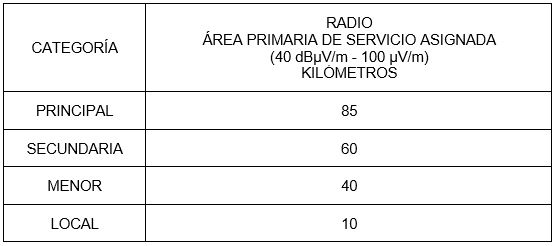
\includegraphics{contenido/img/ej7tab1.JPG}
        \caption{BANDA I-VHF(Canales 2 al 6)}
    \end{center}
\end{table}

\begin{table}[ht]
    \begin{center}
        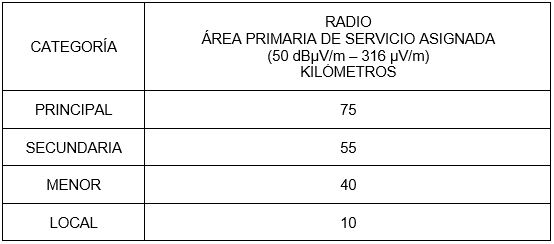
\includegraphics{contenido/img/ej7tab2.JPG}
        \caption{BANDA II-VHF(Canales 7 al 13)}
    \end{center}
\end{table}

\begin{table}[ht]
    \begin{center}
        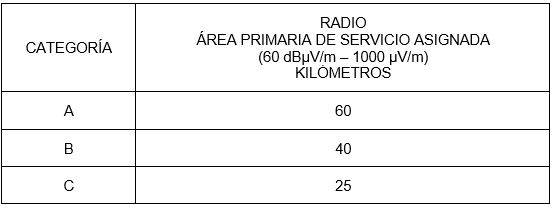
\includegraphics{contenido/img/ej7tab3.JPG}
        \caption{BANDA III-VHF(Canales 21 al 69)}
    \end{center}
\end{table}

\newpage
\section{sistema de Televisión Codificada (STVC)}
Es aquel cuyas emisiones están destinadas a la recepción, previa decodificación, por parte del público abonado al sistema.

\begin{table}[ht]
    \begin{center}
        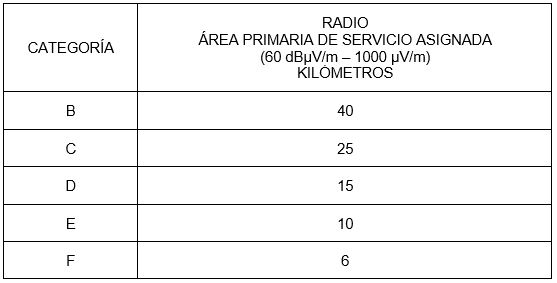
\includegraphics{contenido/img/ej7tab4.JPG}
        \caption{BANDA I-VHF(Canales 2 al 6)}
    \end{center}
\end{table}